\documentclass[a4paper,12pt]{article}
\usepackage[utf8]{inputenc}
\usepackage[english]{babel}
\usepackage{authblk}
\usepackage{graphicx}
\usepackage{mathptmx}
\usepackage[singlespacing]{setspace}
\usepackage[headheight=1in,margin=1in]{geometry}
\usepackage{fancyhdr}
\usepackage{soul}
\usepackage[parfill]{parskip}
\usepackage[colorlinks]{hyperref}
\renewcommand{\headrulewidth}{0pt}
\pagestyle{fancy}
\chead{%
   $5$$^{th}$ International Conference on Computational Social Science IC$^{2}$S$^{2}$\\
   July 17-20, 2019, University of Amsterdam, The Netherlands%
}
%\graphicspath{{images/}}
\title{Are Online Users with Us ? Deep Representation Learning for Political Stance Detection}
\author[1]{Zoya Khan}\author[1]{Priyam Bansal} \author[1]{Mansi Sharma} \author[1]{Rishabh Kaushal} 
\affil[1]{Indira Gandhi Delhi Technical University for Women, New Delhi, India}
% Please leave Author-field blank for blind review and remove information that may identify the author(s)
\date{}
\begin{document}
\maketitle
\thispagestyle{fancy}
%\vspace{-6em}
\vspace{-3em}
\begin{center}
\textbf{\textit{Keywords: Stance detection, Politics, Autoencoder, Online Social Media, Deep Learning}}
%\newline
\end{center}
%\section*{Extended Abstract}

\textbf{Introduction \& Impact}: Many Online Social Media (OSM) platforms in general and Twitter in particular, have become popular online avenues for political discourse. 
Politicians and general public are both active on these platforms and therefore, the problem of understanding people's opinions has become very crucial.
%Among other platforms, Twitter has become a popular choice to express such thoughts, opinions and views among general public and political entities alike.
Prior works \cite{lai2016friends,johnson2016identifying} refer this problem as \textit{stance detection} where the goal is to detect user's opinion about a particular issue.
%\color{red}To Do: Add 1/2 sentences here to describe limitation of these prior approaches, which we plan to address in our work.}
This is the first study that focuses on complex Indian political scenario, where there are numerous political parties.
%and people tweet in many languages, to detect stance of the general public using the context based features of the tweets.
Detecting stance of online users would provide very useful information to political parties, using which they can re-calibrate their political strategies.

\textbf{Data Collection \& Ground Truth}:
%We propose a novel methodology for detecting the political stance of Twitter users based on their online tweeting behaviour. 
We collect tweets related to political parties in the national capital region of Delhi in India, the largest democracy in the world.
Unlike bi-partisan democracies like the USA, India's polity is more complex owing to the prevalence of many political parties catering to the diversities in India. 
For our data collection, we focus on three parties namely, Aam Aadmi Party (AAP), Bhartiya Janta Party (BJP) and the Indian National Congress (INC).
%{\color{red}To Do: How many tweets were collected ? What were the keywords used to collect the tweets ?} 
We search for the target users by tweets which contain certain hashtags like - \#BJP, \#AAP, \#INC, \#politics, \#elections  etc. to identify users who actively tweet about politics and then collected tweets from their timeline to get 3,76,932 tweets. To create ground truth, we manually annotate tweets at two levels. At \textit{first level}, we provide a binary label (0 or 1) depending upon whether the tweet is stance neutral or stance revealing. 
At \textit{second level}, we give six mutually exclusive labels from 1 to 6, indicating Pro-AAP, Pro-BJP, Pro-INC, Anti-AAP, Anti-BJP \& Anti-INC, respectively. 
%We assume that a stance revealing tweet can belong to only one of the six labels.
The annotations were done over a two month period by strictly abiding to a set of annotation guidelines which were formulated for this purpose.

\begin{figure}[h]
\centering
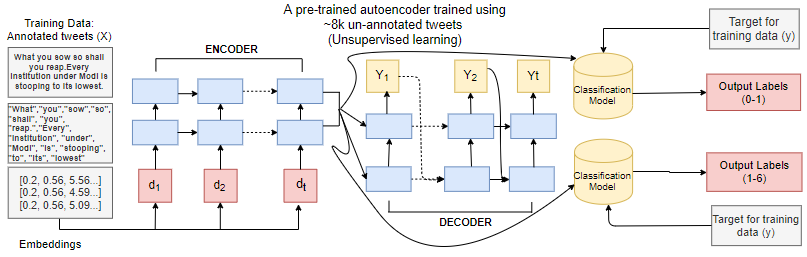
\includegraphics[width=15cm]{IC2S2_Latex_template/images/final5.png}
\caption{%{\color{red} Use one tweet from dataset as example instead of writing generic text like This is first} 
Our model follows a deep learning approach of using an Autoencoder to create tweet-level vectors and then performs a two level classification using these intermediate vectors to detect stance revealing tweets.}
\label{fig:image}
\end{figure}

\textbf{Methodology}:
We follow a two-step methodology based on deep learning. 
In \textit{first step}, the goal is to detect tweets that are stance revealing. 
In \textit{second step}, the goal is to take stance revealing tweet as input and identify the exact stance made in the tweet in terms of three political parties considered in the study. 
We propose to solve the first step in two phases. In first phase, we aim to learn effective representations of user generated information (tweet). In second phase, we pass the learned feature vectors as input to conventional classification algorithms namely Random Forest (RF) , Decision Tree, Naive Bayes and SVM. 
For effective representation learning of first phase, we employ a deep neural network based autoencoder inspired by Sutskever et al. \cite{sutskever2014sequence}. %{\color{red} Cite paper where autoencoder's use was first proposed} to create an intermediate learned representation of the input sequence of words (tweets) in unsupervised manner. 
%This technique produces significantly better results as compared to the earlier two techniques. 
Here we implement an autoencoder which is an unsupervised learning algorithm, used for compressing high dimensional input data to lower dimensions in order to learn a more compact and efficient representation of the input. It then attempts to reconstruct the initial input given this intermediate representation. 

\textbf{Evaluation \& Results}:
We compare our autoencoder based approach with two baselines.
\begin{enumerate}
    \item Word2vec (w2v) Model \cite{mikolov2013efficient}: It is a neural network based model, trained on the vocabulary of the input dataset to generate word vectors. To represent phrase (tweet) level vectors, we take the mean of word vectors as suggested by Mikolov et. al. \cite{mikolov2013distributed}. 
    %{\color{red} To Do: Why this number is coming here? Methodology is written generically. Also add footnotes or references to research paper where this approach was first used.}%
    \item Google Embedding: It is Google's Pre-trained word embeddings created by Mikolov et. al. \cite{mikolov2013distributed} and trained on the Google news data. 
    %We create tweet level vectors as used in approach (1).
    %\item Our third approach %It can also be contextualized as  a  machine  containing  an  Encoder and  a  Decoder. %Autoencoders are increasingly being used in tasks of language modelling, machine translation and other NLP applications as it produces significantly better results than conventional text processing systems.
\end{enumerate}


%{\color{red}To Do: Include complete results table, there is still space.}
\begin{table}[!htbp]
\caption{Scores for all classification models after phase 1}
\medskip
\centering
\begin{tabular}{|p{4.5cm}|p{2cm}|p{2.5cm}|p{2.5cm}|}
\hline
Model&word2vec (Mean)&Google's Pre-trained&Auto Encoder \\
\hline \hline
Naive Bayes & 0.481 & 0.641 & 0.155 \\ 
\hline
Random Forest & 0.774 & 0.759 & 0.849 \\  
\hline
Decision Tree & 0.643  & 0.657 & 0.799 \\
\hline
Support Vector Classifier & 0.774  & 0.759 & 0.849 \\
\hline
\end{tabular}
\label{tab:lab1}
\end{table}

% \begin{table}[!htbp]
% \caption{Scores for all classification models after phase 2}
% \medskip
% \centering
% \begin{tabular}{|p{4.5cm}|p{2cm}|p{2.5cm}|p{2.5cm}|}
% \hline
% Model&word2vec (Mean)&Google's Pre-trained&Auto Encoder \\
% \hline \hline
% Naive Bayes & 0 & 0 & 0 \\ 
% \hline
% Random Forest & 0 & 0 & 0 \\  
% \hline
% Decision Tree & 0 & 0 & 0 \\
% \hline
% Support Vector Classifier & 0 & 0 & 0 \\
% \hline
% \end{tabular}
% \label{tab:lab1}
% \end{table}

\bibliographystyle{IEEEtran}
\bibliography{refer} 

\iffalse
\begin{itemize}
  \cite{}
\end{itemize}
\fi


\vskip 40pt
\end{document}
